\documentclass{standalone}

\usepackage{tikz}
\usetikzlibrary{decorations.pathreplacing}
\usetikzlibrary{shapes.geometric}
\usetikzlibrary{automata}

\begin{document}
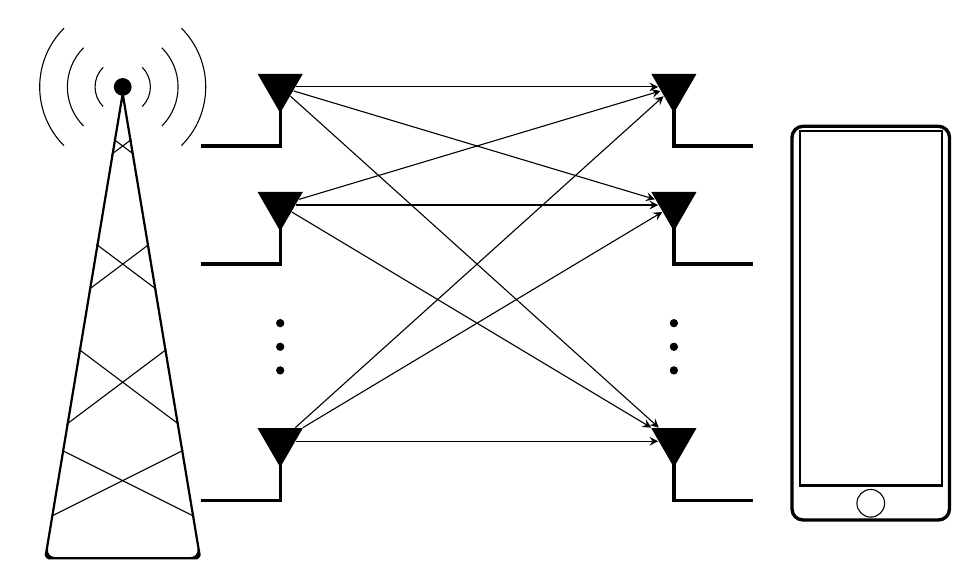
\begin{tikzpicture}[y=1.5cm, >=stealth]
  % \draw[gray, very thin, step=1] (0,0) grid (15,6);
  % \foreach \x in {1,...,15} \node at (\x,0) {\x};
  % \foreach \y in {1,...,6} \node at (0,\y) {\y};
  \begin{scope}
    \clip (0,1) -- (2,1) -- (1,5) -- cycle;
    \draw[rounded corners, draw, ultra thick] (0,1) -- (2,1) -- (1,5) -- cycle;
    \draw (-1,1) -- (2,2) -- (0,3) -- (2,4) -- (0,5) -- (2,5) -- (0,4) -- (2,3) -- (0,2) -- (3,1);
  \end{scope}
  \filldraw(1,5) circle [radius=3pt];
  \draw [decorate,decoration={expanding waves}](1,5) -- +(1.2,0);
  \draw [decorate,decoration={expanding waves}](1,5) -- +(-1.2,0);

  \node[name=antt1,regular polygon,regular polygon sides=3, minimum size = 2pt, fill, shape border rotate=180] at (3,5){};
  \draw[very thick] (antt1.base) |- +(-1,-0.5);
  \node[name=antt2,regular polygon,regular polygon sides=3, minimum size = 2pt, fill, shape border rotate=180] at (3,4){};
  \draw[very thick] (antt2.base) |- +(-1,-0.5);
  \node[name=antt3,regular polygon,regular polygon sides=3, minimum size = 2pt, fill, shape border rotate=180] at (3,2){};
  \draw[very thick] (antt3.base) |- +(-1,-0.5);

  \fill (3,2.8) circle[radius=1.5pt] +(0,0.2) circle[radius=1.5pt] +(0,-0.2) circle[radius=1.5pt];
  \node[name=antr1,regular polygon,regular polygon sides=3, minimum size = 2pt, fill, shape border rotate=180] at (8,5){};
  \draw[very thick] (antr1.base) |- +(1,-0.5);
  \node[name=antr2,regular polygon,regular polygon sides=3, minimum size = 2pt, fill, shape border rotate=180] at (8,4){};
  \draw[very thick] (antr2.base) |- +(1,-0.5);
  \node[name=antr3,regular polygon,regular polygon sides=3, minimum size = 2pt, fill, shape border rotate=180] at (8,2){};
  \draw[very thick] (antr3.base) |- +(1,-0.5); 

  \fill (8,2.8) circle[radius=1.5pt] +(0,0.2) circle[radius=1.5pt] +(0,-0.2) circle[radius=1.5pt];
  
  \draw[->] (antt1) -- (antr1);
  \draw[->] (antt1) -- (antr2);
  \draw[->] (antt1) -- (antr3);
  
  \draw[->] (antt2) -- (antr1);
  \draw[->] (antt2) -- (antr2);
  \draw[->] (antt2) -- (antr3);

  \draw[->] (antt3) -- (antr1);
  \draw[->] (antt3) -- (antr2);
  \draw[->] (antt3) -- (antr3);

  \node[minimum width = 2cm, minimum height=5cm, very thick, rounded corners, draw, rectangle] at (10.5,3) {};
  \node[minimum width = 1.8cm, minimum height=4.5cm, thick, draw, rectangle] at (10.5,3.125) {};
  \draw (10.5,1.475) circle[radius=5pt];
\end{tikzpicture}
\end{document}

%%% Local Variables:
%%% mode: latex
%%% TeX-master: t
%%% End:
